\documentclass{article}
\usepackage{graphicx}
\usepackage[margin=1.5cm]{geometry}
\usepackage{amsmath}

\begin{document}
\twocolumn

\title{Warm Up Exercises: Unit 2, Forces}
\author{Prof. Jordan C. Hanson}

\maketitle

\begin{figure}[ht]
\centering
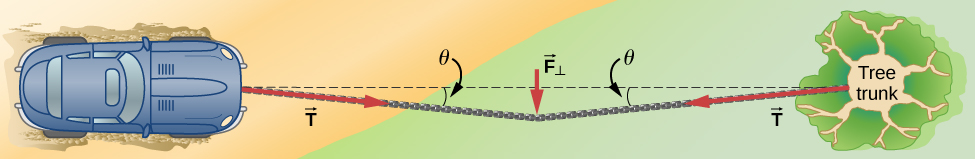
\includegraphics[width=0.49\textwidth]{figures/rope.jpeg}
\caption{\label{fig:1} Person pushes in a direction orthogonal to a rope connecting a car and a tree.}
\end{figure}

\section{Memory Bank}

\begin{enumerate}
\item $\vec{F} = m \vec{a}$ ... Newton's 2nd Law
\item $\vec{a} = d^2\vec{x}/dt^2$ ... Definition of acceleration
\end{enumerate}

\section{Chapter 4 - Forces}

\begin{enumerate}
\item A particle of mass $m$ is falling under the influence of gravity, but experiences a thrust force upwards $\vec{F}_t = kt\hat{j}$, making the net force $\vec{F}_{\rm Net} = kt\hat{j}-mg\hat{j}$.  (a) Express the vertical \textit{velocity} as a function of time, assuming the vertical velocity is $v_0$ at $t=0$. (b) If $v_0 = 3$ m/s, $m = 20$ kg, and $v(10) = 30$ m/s, what is $k$? \\ \vspace{5cm}
\item A 20,000 kg jet fighter lands on an aircraft carrier, moving at 108 km/hr. A tow cable grabs the aircraft and pulls it to a stop in 100 meters. (a) What is the average acceleration? (b) What force does the tow cable extert to stop the jet? \\ \vspace{4cm}
\item Consider Fig. \ref{fig:1}, in which a rope is tied to a tree and a car stuck in mud.  The force is perpendicular to the middle of the rope, $\vec{F}_{\perp}$.  Suppose $\vec{F}_{\perp}$, the left-pointing tension $\vec{T}$, and right-pointing tension $\vec{T}$ all cancel to yield $\vec{F}_{net} = 0$, show that
\begin{equation}
2T\sin\theta = F_{\perp}
\end{equation}
\textit{Hint: it helps if you think of the tension vectors as pointing the opposite direction as shown in Fig. 1.} \\ \vspace{4cm}
\item What is the tension in the rope if we find an angle $\theta = 10$ degrees, and $F_{\perp} = 500$ N?
\end{enumerate}

\end{document}
